% =====================================================================
%  Plateforme de gestion de thèse CIFRE
%  Réglementation, acteurs, état de l'art, cahier des charges,
%  sécurité et choix techniques
%  Auteur : Adya Sarr — version du 12 novembre 2026
%  Compilation : pdflatex (deux passes) ou latexmk -pdf
% =====================================================================
\documentclass[11pt,a4paper]{article}

\usepackage[utf8]{inputenc}
\usepackage[T1]{fontenc}
\usepackage{lmodern}
\IfFileExists{french.ldf}{\usepackage[french]{babel}}{\usepackage[english]{babel}}
\usepackage[margin=2.2cm]{geometry}
\usepackage{microtype}
\usepackage{array,tabularx,booktabs}
\usepackage{ragged2e}
\usepackage[table]{xcolor}
\usepackage{enumitem}
\usepackage{amssymb}
\usepackage{tikz}
\usetikzlibrary{positioning,arrows.meta,fit,backgrounds}
\usepackage[most]{tcolorbox}
\usepackage{fancyhdr}
\usepackage{hyperref}

\definecolor{bleu}{HTML}{1F4E79}
\definecolor{gris}{HTML}{F0EFEC}
\definecolor{alerte}{HTML}{FBEBEB}
\hypersetup{colorlinks=true,linkcolor=bleu,urlcolor=bleu,citecolor=bleu,
  pdftitle={Plateforme de gestion de thèse CIFRE},pdfauthor={Adya Sarr}}

\newcolumntype{L}{>{\RaggedRight\arraybackslash}X}
\newcolumntype{P}[1]{>{\RaggedRight\arraybackslash}p{#1}}
\renewcommand{\arraystretch}{1.25}
\setlist{itemsep=2pt,topsep=4pt}

\newtcolorbox{apretenir}[1][À retenir]{colback=gris,colframe=bleu,
  fonttitle=\bfseries,title=#1,boxrule=0.6pt,arc=2pt}
\newtcolorbox{question}[1][Question ouverte]{colback=alerte,colframe=red!50!black,
  fonttitle=\bfseries,title=#1,boxrule=0.6pt,arc=2pt}

\pagestyle{fancy}
\fancyhf{}
\lhead{\small Plateforme de gestion de thèse CIFRE}
\rhead{\small A. Sarr}
\cfoot{\thepage}

\title{\textbf{Plateforme de gestion de thèse CIFRE}\\[4pt]
\large Réglementation, acteurs, état de l'art, cahier des charges,\\
sécurité et choix techniques}
\author{Adya Sarr\\ \small Thèse CIFRE STMicroelectronics (Rousset) -- LIRMM (équipe ARTHEMIS)\\ \small ED I2S, Université de Montpellier}
\date{12 novembre 2026}

\begin{document}
\maketitle
\thispagestyle{empty}

\begin{abstract}
Aucune plateforme existante ne couvre une thèse CIFRE de bout en bout : ADUM gère
le volet universitaire, l'ANRT le volet financement, et rien ne relie au quotidien
les trois parties (doctorant, entreprise, laboratoire). Ce document rassemble le
cadre réglementaire français, les obligations propres à la CIFRE, les acteurs
impliqués, un calendrier type, un état de l'art des plateformes de suivi doctoral,
les conférences du domaine, puis le cahier des charges d'une plateforme dédiée,
son modèle de sécurité (chiffrement de bout en bout des données confidentielles,
cryptographie post-quantique hybride) et le choix des technologies pour la coder.
\end{abstract}

\tableofcontents
\newpage

% =====================================================================
\section{En bref}
% =====================================================================

Contexte retenu : thèse CIFRE employée par STMicroelectronics (Rousset),
laboratoire académique LIRMM (équipe ARTHEMIS, Montpellier), école doctorale I2S
de l'Université de Montpellier, début prévu en mars 2027, sujet : attaques
physiques contre la cryptographie post-quantique.

Quatre contraintes structurent tout le reste :
\begin{itemize}
  \item \textbf{Réglementaire} : l'arrêté du 25 mai 2016 modifié en 2022 impose un
  comité de suivi annuel, une convention de formation, un portfolio et une
  formation à l'intégrité scientifique.
  \item \textbf{CIFRE} : un rapport annuel à l'ANRT cosigné par les trois parties,
  et un contrat de collaboration qui fixe la propriété intellectuelle et la
  confidentialité.
  \item \textbf{Sécurité} : le LIRMM est en zone à régime restrictif (ZRR) et le
  sujet touche la sécurité de composants industriels. Les données peuvent être
  sensibles : l'hébergement doit être validé par ST et le LIRMM avant tout
  développement.
  \item \textbf{Sobriété} : la plateforme échoue si les encadrants doivent y passer
  du temps ; elle doit leur pousser l'information.
\end{itemize}

% =====================================================================
\section{Cadre réglementaire du doctorat}
% =====================================================================

Le texte de référence est
l'\href{https://www.legifrance.gouv.fr/loda/id/JORFTEXT000032587086}{arrêté du 25 mai 2016}
fixant le cadre national de la formation doctorale, modifié par
l'\href{https://www.legifrance.gouv.fr/jorf/id/JORFTEXT000046228965}{arrêté du 26 août 2022},
en vigueur depuis le 1\textsuperscript{er} septembre 2022. Chaque obligation
ci-dessous devient un objet suivi dans la plateforme.

\begin{center}\small
\begin{tabularx}{\linewidth}{P{3.6cm} P{1.6cm} L P{2.2cm}}
\toprule
\textbf{Obligation} & \textbf{Article} & \textbf{Ce que cela implique} & \textbf{Qui}\\
\midrule
Charte du doctorat et convention individuelle de formation & art.~12 &
Signées dans ADUM à l'inscription. La convention fixe le sujet, le financement, le
calendrier, l'encadrement, le projet professionnel et la valorisation (publication,
confidentialité, PI). Révisable à chaque réinscription. & Doctorant, directeur, ED\\
Inscription puis réinscription annuelle & art.~11 &
Aucune réinscription sans l'avis du comité de suivi. & Doctorant, ED\\
Comité de suivi individuel (CSI) & art.~13 &
Entretien annuel en trois temps : avancement, échange avec le doctorant seul,
échange avec la direction seule. Au moins un spécialiste, si possible un membre
extérieur, et un non-spécialiste. & Comité, ED\\
Plan individuel de formation et portfolio & art.~12 et 15 &
Formations, publications, compétences, enseignement. La charte I2S recommande
environ 100~h de formation sur le doctorat. & Doctorant\\
Formation à l'éthique et à l'intégrité scientifique & art.~3 &
Obligatoire pour soutenir. & Doctorant\\
Durée & art.~14 &
Trois ans en équivalent temps plein ; au-delà, prolongation dérogatoire sur demande
motivée, après avis du CSI. & Doctorant, directeur, ED\\
Soutenance & art.~17 à 19 &
Au moins deux rapporteurs habilités, autorisation du chef d'établissement. Soutenance
publique ; huis clos exceptionnel si confidentialité avérée. & ED, jury\\
Serment du docteur & art.~16 &
Prêté après l'admission : engagement à l'intégrité scientifique. & Docteur\\
Dépôt et diffusion & art.~24 et 25 &
PDF/A validé par \href{https://facile.cines.fr}{FACILE (CINES)}, envoi vers STAR
(ABES), signalement sur theses.fr ; version corrigée sous trois mois si le jury
l'exige. & Docteur, bibliothèque\\
\bottomrule
\end{tabularx}
\end{center}

\begin{apretenir}
\begin{itemize}[leftmargin=*]
  \item \textbf{Le CSI est l'échéance pivot de chaque année.} Le rapport du doctorant
  est souvent exigé deux semaines avant l'entretien ; l'avis est déposé dans ADUM.
  \item \textbf{La convention de formation est vivante.} Les objectifs annuels de la
  plateforme en sont la déclinaison opérationnelle.
  \item \textbf{La confidentialité se décide tôt.} Une thèse CIFRE sur la sécurité de
  puces peut nécessiter un embargo ou un huis clos : à prévoir dès la convention.
\end{itemize}
\end{apretenir}

\begin{question}
L'Université de Montpellier ouvre les inscriptions en 1\textsuperscript{re} année de
juillet à décembre
(\href{https://ed461.edu.umontpellier.fr/files/2025/08/IDD_Calendrier-Inscriptions-Administratives_2025-2026.pdf}{calendrier 2025--2026}).
Pour un début en mars 2027, confirmer avec l'ED I2S la procédure d'inscription en
cours d'année.
\end{question}

% =====================================================================
\section{Le dispositif CIFRE}
% =====================================================================

La CIFRE est une subvention de l'État versée par l'ANRT à l'entreprise qui emploie le
doctorant, en contrepartie d'un projet de recherche mené avec un laboratoire
académique. Elle repose sur deux contrats distincts : la convention ANRT--entreprise
(le financement) et le contrat de collaboration entreprise--laboratoire
(encadrement, PI, confidentialité), qui n'implique pas l'ANRT.

\begin{center}\small
\begin{tabularx}{\linewidth}{P{4.2cm} L}
\toprule
\textbf{Élément} & \textbf{Valeur ou règle}\\
\midrule
Subvention ANRT à l'entreprise & 14\,000~€ par an pendant 3 ans\\
Salaire minimum (2026) & 27\,600~€ brut par an\\
Contrat de travail & CDI ou CDD de 36 mois, convention collective de l'entreprise\\
Éligibilité du doctorant & Ne pas avoir travaillé plus de 9 mois pour l'entreprise avant le dépôt (stages et apprentissage exclus)\\
Répartition du temps & 100\,\% sur la thèse, partagé entreprise / laboratoire ; souvent 70/30, au moins 20\,\% au laboratoire selon l'ANRT\\
Laboratoire & Rattaché à l'école doctorale d'inscription\\
Sélection & Comité d'évaluation et de suivi (CES) mensuel, deux expertises (scientifique et socio-économique), instruction de 3 à 6 mois\\
Date d'effet & Au mieux le 15 du mois suivant le CES\\
Suivi & Rapport d'activité annuel signé par l'entreprise, le laboratoire et le doctorant, remis à l'ANRT\\
Versement & Conditionné à la signature du contrat de collaboration\\
\bottomrule
\end{tabularx}
\end{center}

\noindent Sources :
\href{https://static.psl.eu/sites/default/files/2026-07/Webinaire\%20CIFRE\%20COFRA\%2007.04.26.pdf}{webinaire CIFRE PSL (avril 2026)},
\href{https://ed-lls.parisnanterre.fr/medias/fichier/presentation-cifre-cofra_1776946105660-pdf}{présentation CIFRE Paris Nanterre (2026)}.

\paragraph{Conséquences pour la plateforme.}
\begin{itemize}
  \item \textbf{Deux calendriers parallèles} : l'année CIFRE court depuis la date
  d'effet, l'année universitaire de septembre à août ; rapport ANRT et CSI tombent à
  des moments différents.
  \item \textbf{Suivi du temps entreprise / laboratoire} : la répartition est
  contractuelle ; un journal des jours à Rousset et à Montpellier la documente.
  \item \textbf{Circuit de validation avant publication} : chez un industriel, un
  article passe souvent par une relecture interne, voire un dépôt de brevet. Ce
  délai doit être décompté des deadlines.
  \item \textbf{Alerte précoce} : si un rapport révèle une difficulté, l'ANRT saisit le
  CES ; mieux vaut rendre les signaux faibles visibles bien avant.
\end{itemize}

% =====================================================================
\section{Acteurs et organismes}
% =====================================================================

Onze acteurs interviennent ; seuls les cinq premiers ont besoin d'un compte.

\begin{center}\small
\begin{tabularx}{\linewidth}{P{3.8cm} L P{3.6cm}}
\toprule
\textbf{Acteur} & \textbf{Rôle dans la thèse} & \textbf{Plateforme}\\
\midrule
Doctorant (salarié ST) & Porte le projet, met à jour l'avancement & Administrateur\\
Directeur de thèse (LIRMM, HDR) & Responsable scientifique devant l'ED, signe les rapports & Lecture, commentaires, validation\\
Co-encadrant(s) LIRMM & Encadrement scientifique au quotidien & Lecture, commentaires\\
Tuteur industriel (ST Rousset) & Suivi entreprise, cosigne le rapport ANRT & Lecture, validation des publications\\
Membres du CSI & Avis annuel sur la réinscription & Accès temporaire au dossier CSI\\
École doctorale I2S & Inscription, formations, CSI, soutenance & Aucun compte (tout passe par \href{https://www.adum.fr}{ADUM})\\
LIRMM, UMR 5506 & Laboratoire d'accueil ; dépôt obligatoire sur \href{https://www.lirmm.fr/?p=1097}{HAL-LIRMM} ; SeminDocs & Export vers HAL\\
Fonctionnaire sécurité défense (FSD) & Autorise l'accès à la ZRR & Contrainte d'hébergement\\
ST, RH et juridique & Employeur, confidentialité, PI & Règles de confidentialité\\
ANRT & Gestion de la CIFRE pour le ministère & Génération du rapport\\
ABES / CINES & theses.fr, STAR, archivage pérenne & En fin de thèse\\
\bottomrule
\end{tabularx}
\end{center}

\subsection*{La ZRR, un point d'attention propre à ce cas}
Les zones à régime restrictif relèvent de la protection du potentiel scientifique et
technique de la nation (PPST). L'accès exige un avis du FSD et du ministère ; le décret
du 14 mai 2024 et
l'\href{https://armement.defense.gouv.fr/sites/default/files/2025-05/Instruction\%20interminist\%C3\%A9rielle_20250428_PPST.pdf}{instruction interministérielle du 28 avril 2025}
en fixent les règles. Selon le
\href{https://www.snesup.fr/sites/default/files/2025-11/recherche_snesup-ndeg-738pp22-23.pdf}{SNESUP},
le délai moyen était de 34 jours pour un ressortissant étranger contre 16 pour un
Français. Les informations produites en ZRR peuvent être des \emph{informations à
régime restrictif} ; l'ANSSI publie un
\href{https://armement.defense.gouv.fr/sites/default/files/2022-02/guide_ANSSI_protection_numerique_PSTN_juin_2018.pdf}{guide de protection des SI en ZRR}.
Un hébergement grand public (Notion, Trello, Vercel) est donc probablement exclu pour
le contenu scientifique.

% =====================================================================
\section{Calendrier type (début mars 2027)}
% =====================================================================

Estimations à caler une fois la date d'effet ANRT connue. Chaque ligne devient un
jalon avec rappels à J-60, J-30 et J-7.

\begin{center}\small
\begin{tabularx}{\linewidth}{P{2.9cm} L P{2.8cm} P{1.9cm}}
\toprule
\textbf{Période} & \textbf{Jalon} & \textbf{Responsable} & \textbf{Base}\\
\midrule
Avant début & Dossier ANRT, contrat de travail ST, avis FSD, contrat de collaboration ST--LIRMM & ST, LIRMM, doctorant & CIFRE, PPST\\
Mars 2027 (M0) & Inscription ADUM, charte et convention signées, plan de formation, objectifs année 1 & Doctorant, directeur, ED & art.~11--12\\
M1--M6 & État de l'art, prise en main du banc de mesure ST, premiers résultats & Doctorant & --\\
Sept. 2027 & 1\textsuperscript{re} réinscription ; un CSI peut être exigé malgré six mois seulement & ED & art.~13 (à confirmer)\\
Mars 2028 (M12) & Rapport ANRT n\textsuperscript{o}1 ; bilan des objectifs année 1 & Doctorant, tuteur, directeur & CIFRE\\
Été 2028 & CSI année 2 puis réinscription & Comité, ED & art.~13\\
M12--M24 & Premier article (CASCADE ou TCHES), environ 35~h de formation & Doctorant & charte I2S\\
Mars 2029 (M24) & Rapport ANRT n\textsuperscript{o}2 ; plan du manuscrit & Doctorant, encadrants & CIFRE\\
Été 2029 & CSI année 3 ; vérification des 100~h et de l'intégrité & Comité, ED & art.~3, 13\\
Sept. 2029 -- janv. 2030 & Rédaction ; jury et rapporteurs proposés environ trois mois avant & Doctorant, directeur & art.~17--18\\
$\sim$ janv. 2030 & Envoi aux rapporteurs ; rapports au moins un mois avant & ED & art.~17\\
Mars 2030 (M36) & Soutenance, serment, fin de CIFRE, rapport final & Jury, doctorant, ST & art.~16--19\\
$\leq$ 3 mois après & Dépôt définitif PDF/A dans ADUM, envoi vers STAR & Docteur & art.~24--25\\
\bottomrule
\end{tabularx}
\end{center}

% =====================================================================
\section{État de l'art des plateformes}
% =====================================================================

Les outils existants se répartissent en trois familles. Aucun ne gère le partenariat
tripartite d'une CIFRE ni la confidentialité industrielle : ils sont conçus pour
l'institution, pas pour le doctorant et ses encadrants.

\subsection{Outils officiels français}
\begin{center}\small
\begin{tabularx}{\linewidth}{P{3.2cm} L L}
\toprule
\textbf{Outil} & \textbf{Ce qu'il fait} & \textbf{Ce qu'il ne fait pas}\\
\midrule
\href{https://www.adum.fr}{ADUM} & Inscriptions, charte et convention, CSI, catalogue de formations, portfolio, déclaration de soutenance, envoi vers STAR & Objectifs, réunions, volet entreprise, conférences\\
\href{https://offres-et-candidatures-cifre.anrt.asso.fr/}{Plateforme ANRT} & Offres, dépôt du dossier, rapports & Pilotage quotidien\\
\href{https://hal.science}{HAL}, theses.fr & Archive ouverte, signalement des thèses & Publications confidentielles\\
\bottomrule
\end{tabularx}
\end{center}

\subsection{Plateformes institutionnelles étrangères}
\begin{center}\small
\begin{tabularx}{\linewidth}{P{3.4cm} P{3.2cm} L}
\toprule
\textbf{Plateforme} & \textbf{Origine} & \textbf{Idée à reprendre}\\
\midrule
\href{https://studies.helsinki.fi/instructions/article/thessa}{Thessa} & Univ. d'Helsinki & Plan d'encadrement commun, projet mis à jour par le doctorant, rapports annuels pour le comité. Le plus proche du besoin\\
\href{https://skillsforge.net}{SkillsForge} & Royaume-Uni & Comptes-rendus de réunions saisis et validés, bilan des compétences\\
\href{https://www.haplo.com/phd-manager}{Haplo PhD Manager} & Royaume-Uni & Registre central des réunions, tableaux de bord\\
\href{https://www.utwente.nl/en/service-portal/research-support/phd-engd-programmes-tgs/doctorate-phdengd-monitoring-system}{Doctorate} & Univ. de Twente & Rapport d'avancement une semaine avant l'évaluation, planning mis à jour\\
\href{https://studenthub.city.ac.uk/help-and-support/doctoral-college/research-and-progress}{Research and Progress} & City, Univ. of London & Comptes-rendus tenus conjointement, encadrants externes inclus\\
\href{https://hsd.ardascience.com/index.php/journal/article/download/1623/264/5253}{ProGRess} & Bournemouth Univ. & Développé en interne en méthode agile : retour d'expérience utile\\
\href{https://phdquest.swisstph.ch/}{PhD Workflow Tracker} & Swiss TPH & Phases de l'arrivée aux anciens, échéances\\
\href{https://digiicampus.com/phd-management/}{Digiicampus} & Inde (commercial) & Workflows configurables par rôle\\
\bottomrule
\end{tabularx}
\end{center}

\subsection{Outils généralistes détournés}
Trello, GanttPro, Notion, OpenProject ou GitLab servent souvent aux doctorants. Ils
sont souples mais ignorent le CSI, le rapport ANRT et les rôles d'encadrement, et la
plupart sont hébergés hors de France.

\subsection{Ce que dit la recherche}
\begin{itemize}
  \item La revue de \href{https://doi.org/10.28945/4113}{Sverdlik et al.\ (2018)} place la
  relation d'encadrement et la clarté des attentes parmi les principaux facteurs
  d'achèvement et de bien-être.
  \item \href{https://ajet.org.au/index.php/AJET/article/download/8615/2025/30010}{Fanshawe et Barton (2023)}
  montrent qu'un environnement numérique aide surtout l'autonomie du doctorant et la
  communication avec les encadrants.
  \item Une \href{https://www.journals.eanso.org/index.php/eajes/article/view/1844}{étude à l'Université de Nairobi}
  constate un faible usage des outils numériques en encadrement et recommande un
  modèle hybride.
\end{itemize}

% =====================================================================
\section{Conférences et revues du domaine}
% =====================================================================

Cibles principales : TCHES/CHES, CASCADE et PQCrypto. Dates relevées en novembre 2026 ;
certaines proviennent d'agrégateurs et sont à confirmer sur les sites officiels.

\begin{center}\small
\begin{tabularx}{\linewidth}{P{2.6cm} P{3.3cm} P{3.2cm} L}
\toprule
\textbf{Venue} & \textbf{Prochaine échéance} & \textbf{Événement} & \textbf{Intérêt}\\
\midrule
\href{https://easychair.org/cfp/pqcrypto2027}{PQCrypto 2027} & Résumé 17 nov.\ 2026, article 24 nov.\ 2026 & 12--14 mai 2027, Waterloo & Cœur de sujet ; trop tôt pour cette édition\\
\href{https://tches.iacr.org/index.php/TCHES/submission}{TCHES / CHES 2027} & 15 janv., avril, juil., oct. & 6--9 sept.\ 2027, Cancún & Cible principale\\
\href{https://cascade-conference.org/}{CASCADE 2027} & Deux sessions (été, hiver), à vérifier & Avril 2027, Stuttgart (à confirmer) & Fusion COSADE + CARDIS ; idéal pour un premier article\\
\href{https://rwc.iacr.org/}{Real World Crypto} & Exposés vers mi-décembre & Début avril 2027, Seattle & Atelier Real World PQC ; bourses étudiantes\\
PKC 2027 & Passée (août 2026) & 1\textsuperscript{er}--4 mars 2027, Taipei & Secondaire\\
Eurocrypt 2027 & Passée (17 sept.\ 2026) & 11--15 avril 2027, Eindhoven & Assister\\
Crypto, Asiacrypt & Vers février / mai & Août / décembre & Résultat fort de cryptanalyse\\
ACNS 2027 & Passée (sept.\ 2026) & 28 juin -- 1\textsuperscript{er} juil.\ 2027, Egham & Secondaire\\
\href{https://www.date-conference.com/call-for-papers}{DATE 2027} & Oct.\ 2026 à févr.\ 2027 & 2027, Europe & Culture ST et microélectronique\\
\bottomrule
\end{tabularx}
\end{center}

\noindent À confirmer côté France : Journées Codage et Cryptographie (C2) et
événements du \href{https://gdr-securite.irisa.fr/}{GDR Sécurité informatique}.
Sources automatisables : le
\href{https://www.iacr.org/events/eventsbysubmission.php4}{calendrier IACR} (flux
iCalendar) et \href{https://sec-deadlines.github.io}{sec-deadlines} (licence MIT).

% =====================================================================
\section{Cahier des charges}
% =====================================================================

\subsection{Rôles et droits}
\begin{center}\small\setlength{\tabcolsep}{4pt}
\begin{tabularx}{\linewidth}{P{2.6cm} P{2.0cm} P{1.8cm} P{2.1cm} P{1.8cm} L}
\toprule
\textbf{Rôle} & \textbf{Objectifs} & \textbf{Réunions} & \textbf{Documents} & \textbf{Admin./RH} & \textbf{Valide}\\
\midrule
Doctorant & Écrire & Écrire & Écrire & Écrire & --\\
Directeur de thèse & Commenter & Écrire & Lire, commenter & Lire & Objectifs, CSI, ANRT\\
Co-encadrant LIRMM & Commenter & Écrire & Lire, commenter & -- & --\\
Tuteur ST & Commenter & Écrire & Lire, commenter & Partie CIFRE & ANRT, publications\\
Membre du CSI & Dossier CSI & -- & Rapport CSI & -- & Avis CSI\\
Invité & -- & Une réunion & Projet partagé & -- & --\\
\bottomrule
\end{tabularx}
\end{center}

Chaque document porte un \textbf{niveau de confidentialité} : \emph{public},
\emph{interne LIRMM}, \emph{interne ST}, \emph{confidentiel ST--LIRMM}. Les droits se
déduisent à la fois du rôle et de ce niveau (section~\ref{sec:securite}).

\subsection{Modules}
\begin{enumerate}
  \item \textbf{Dossier administratif.} Liste de contrôle des pièces (contrat de
  travail, convention CIFRE, contrat de collaboration, avis FSD, inscription ADUM,
  charte, convention de formation), chacune avec responsable, statut, date. La thèse
  passe à « active » quand tout est coché par les concernés.
  \item \textbf{Comptes et invitations.} Invitation par courriel avec rôle et
  structure ; authentification forte obligatoire ; journal des accès.
  \item \textbf{Objectifs et indicateurs.} Objectifs par année, rattachés à la
  convention de formation ; critère de réussite, échéance, statut, historique des
  révisions (un objectif abandonné reste visible avec sa raison). Tableau de bord :
  taux d'atteinte par année, retards, tendance.
  \item \textbf{Réunions et présentations.} Points hebdomadaires, comités de pilotage,
  CSI ; ordre du jour, compte-rendu, décisions, actions assignées ; présentations à
  faire (SeminDocs, équipe ST, conférences).
  \item \textbf{Conférences.} Import automatique des deadlines ; pour chaque cible :
  objectif, article visé, délai de relecture ST décompté à rebours, budget, statut.
  \item \textbf{Déplacements Rousset--Montpellier.} Calendrier des séjours au LIRMM,
  ordre de mission, hébergement, compteur de temps entreprise / laboratoire ;
  trajets en train, vélo sur place.
  \item \textbf{Rapports générés.} Rapport CSI et rapport annuel ANRT pré-remplis
  depuis les objectifs, réunions et publications ; export PDF (via LaTeX) ou Word.
  \item \textbf{Portfolio et formations.} Compteur vers les 100~h, intégrité
  scientifique, publications (export HAL et BibTeX), enseignement, projet
  professionnel.
\end{enumerate}

\subsection{Suggestions complémentaires}
\begin{center}\small
\begin{tabularx}{\linewidth}{r P{5.6cm} L}
\toprule
\# & \textbf{Fonction} & \textbf{Pourquoi}\\
\midrule
1 & Validation des publications par ST, délai décompté avant chaque deadline & Première cause de deadline manquée en CIFRE\\
2 & Journal de bord (expériences, mesures, idées, échecs) & Matière des rapports et du manuscrit, traçabilité\\
3 & Registre des décisions & Évite les malentendus ST--LIRMM\\
4 & Registre des risques & Anticiper un avenant ou une réorientation\\
5 & Liens Zotero, Overleaf ou Git & Avancement du manuscrit par chapitre\\
6 & Inventaire des données de mesure (traces) & Plan de gestion des données ; les traces ST ne sortent pas\\
7 & Suivi de l'anglais scientifique & Toutes les conférences cibles sont en anglais\\
8 & Projet professionnel et réseau & Exigé par la convention de formation\\
9 & Point bien-être privé et facultatif & Relation d'encadrement et achèvement sont liés\\
10 & Export « dossier de soutenance » & Prêt pour ADUM\\
\bottomrule
\end{tabularx}
\end{center}

\noindent \textbf{À ne pas faire :} dupliquer ADUM. La plateforme prépare et archive ;
ADUM enregistre.

% =====================================================================
\section{Sécurité et cryptographie}\label{sec:securite}
% =====================================================================

La sécurité est une exigence de premier rang : la plateforme manipule des données
personnelles, des résultats non publiés, des informations couvertes par le secret
industriel de ST et, potentiellement, des informations à régime restrictif issues
de la ZRR. Le principe directeur est simple : \textbf{chiffrer partout où une
donnée peut être lue par quelqu'un qui n'en a pas le droit}, y compris
l'administrateur du serveur pour les documents les plus sensibles.

\begin{apretenir}[Règle d'or]
Ne jamais implémenter soi-même une primitive ni un protocole. Utiliser des
bibliothèques auditées (libsodium, \texttt{pyca/cryptography}, OpenSSL~3.5+,
liboqs pour le post-quantique) et des constructions standard. La politique de
sécurité des systèmes d'information (PSSI) de ST et du LIRMM prime sur ce document.
\end{apretenir}

\subsection{Modèle de menace}
\begin{center}\small
\begin{tabularx}{\linewidth}{P{4.2cm} L P{4.6cm}}
\toprule
\textbf{Menace} & \textbf{Exemple} & \textbf{Contre-mesure principale}\\
\midrule
Interception réseau & Wi-Fi de conférence, proxy & TLS 1.3 avec échange de clés hybride post-quantique\\
Vol d'identifiants & Hameçonnage d'un encadrant & Clés d'accès FIDO2 / WebAuthn, sans mot de passe\\
Escalade de droits & Un invité lit un document ST & Contrôle d'accès côté serveur, refus par défaut\\
Compromission du serveur & Faille applicative, administrateur curieux & Chiffrement applicatif par enveloppe ; chiffrement de bout en bout pour le niveau confidentiel\\
Vol de sauvegarde & Disque ou bucket exposé & Sauvegardes chiffrées côté client\\
Falsification & Modifier une validation a posteriori & Signatures numériques et journal chaîné\\
« Récolter maintenant, déchiffrer plus tard » & Trafic enregistré, cassé par un futur ordinateur quantique & Cryptographie hybride classique + post-quantique\\
\bottomrule
\end{tabularx}
\end{center}

\subsection{Données en transit}
\begin{itemize}
  \item TLS~1.3 uniquement, HSTS, certificats renouvelés automatiquement.
  \item \textbf{Échange de clés hybride} \texttt{X25519MLKEM768} (X25519 + ML-KEM-768,
  FIPS~203), disponible dans OpenSSL~3.5 et les navigateurs récents : protège dès
  aujourd'hui contre le déchiffrement futur. Une démonstration cohérente avec le sujet
  de thèse.
  \item Les courriels de notification ne contiennent \textbf{aucun contenu} : un lien
  vers la plateforme seulement.
\end{itemize}

\subsection{Authentification et sessions}
\begin{itemize}
  \item Clés d'accès FIDO2 / WebAuthn comme méthode principale ; TOTP en secours.
  \item Si des mots de passe existent : hachage \textbf{Argon2id} avec sel unique.
  \item Option SSO : fédération Éducation-Recherche (Renater) pour le LIRMM, SSO
  d'entreprise pour ST, via OpenID Connect ou SAML (à valider avec les services
  informatiques).
  \item Cookies \texttt{Secure}, \texttt{HttpOnly}, \texttt{SameSite=Strict} ; sessions
  courtes ; ré-authentification pour toute validation ou changement de droits.
\end{itemize}

\subsection{Autorisation}
Contrôle d'accès à base de rôles (RBAC) combiné à des attributs (ABAC) : une requête
n'aboutit que si le rôle \emph{et} le niveau de confidentialité du document
l'autorisent. Vérification systématique côté serveur, refus par défaut, tests
automatisés de chaque règle.

\subsection{Données au repos : chiffrement par enveloppe}
\begin{itemize}
  \item Disques chiffrés (LUKS) : protection minimale contre le vol physique.
  \item \textbf{Chiffrement applicatif} des champs et fichiers sensibles : chaque
  document reçoit une clé de données (DEK) aléatoire ; contenu chiffré en
  AES-256-GCM ou XChaCha20-Poly1305 (AEAD), avec les métadonnées (identifiant,
  niveau) en données associées pour empêcher les substitutions.
  \item La DEK est chiffrée par une clé maîtresse (KEK) propre à chaque niveau de
  confidentialité, conservée dans un gestionnaire de secrets (HashiCorp Vault ou
  OpenBao), idéalement adossé à un HSM ; rotation périodique des KEK.
\end{itemize}

\subsection{Chiffrement de bout en bout du niveau « confidentiel ST--LIRMM »}
Pour les documents les plus sensibles, le serveur ne doit jamais voir le clair.
\begin{itemize}
  \item Chaque membre possède une paire de clés générée dans son navigateur (clé
  privée protégée par sa clé d'accès ou une phrase de passe).
  \item Un document est chiffré côté client avec une DEK, elle-même encapsulée pour
  chaque destinataire autorisé : X25519 aujourd'hui, \textbf{hybride X25519 +
  ML-KEM-768} dès que les bibliothèques navigateur le permettent.
  \item Ajout d'un membre : ré-encapsulation de la DEK ; retrait : rotation de la DEK.
  \item Contrepartie assumée : pas de recherche plein texte côté serveur sur ces
  documents.
\end{itemize}

\subsection{Intégrité, signatures et traçabilité}
\begin{itemize}
  \item Chaque \textbf{validation} (objectif, rapport CSI, rapport ANRT, publication)
  est signée par la clé du validateur : Ed25519, puis signature hybride Ed25519 +
  \textbf{ML-DSA-65} (FIPS~204).
  \item \textbf{Journal d'audit chaîné} en ajout seul : chaque entrée contient le
  haché SHA-256 (ou SHA3-256) de la précédente ; l'empreinte du dernier bloc est
  signée chaque jour. Toute modification rétroactive devient détectable.
  \item Horodatage des documents finaux possible par un service RFC~3161.
\end{itemize}

\subsection{Sauvegardes, secrets et chaîne logicielle}
\begin{itemize}
  \item Sauvegardes chiffrées côté client (restic ou BorgBackup), règle 3-2-1,
  stockage en France, restauration testée chaque trimestre.
  \item Aucun secret dans Git ; secrets injectés depuis le gestionnaire ; rotation.
  \item Analyse des dépendances (pip-audit ou npm audit, Renovate), analyse statique
  (Semgrep, Bandit), tests dynamiques (OWASP ZAP) dans l'intégration continue.
  \item Référentiel de vérification : \textbf{OWASP ASVS niveau~2} ; recommandations de
  l'ANSSI.
  \item Fichiers déposés : contrôle du type et de la taille, analyse antivirus
  (ClamAV), service depuis un domaine séparé.
  \item RGPD : données minimales, registre de traitement, durée de conservation fixée,
  journaux pseudonymisés.
\end{itemize}

\subsection{Synthèse des primitives}
\begin{center}\small
\begin{tabularx}{\linewidth}{P{4.0cm} P{5.2cm} L}
\toprule
\textbf{Usage} & \textbf{Choix} & \textbf{Bibliothèque}\\
\midrule
Transport & TLS 1.3, \texttt{X25519MLKEM768} & OpenSSL 3.5+, Caddy ou Nginx\\
Mots de passe & Argon2id & \texttt{argon2-cffi}, libsodium\\
Chiffrement symétrique & AES-256-GCM, XChaCha20-Poly1305 & \texttt{pyca/cryptography}, libsodium\\
Encapsulation de clés & X25519 + ML-KEM-768 (hybride) & libsodium, liboqs\\
Signatures & Ed25519 + ML-DSA-65 (hybride) & libsodium, liboqs\\
Hachage & SHA-256, SHA3-256 & bibliothèque standard\\
Gestion des clés & Vault / OpenBao, HSM si disponible & --\\
\bottomrule
\end{tabularx}
\end{center}

% =====================================================================
\section{En quoi coder la plateforme}
% =====================================================================

\paragraph{Recommandation : Python avec Django, PostgreSQL et htmx.}
\begin{itemize}
  \item \textbf{Python} est le langage le plus probable de ton quotidien de
  cryptographe (SageMath, scripts d'analyse de traces) : une seule langue pour la
  thèse et la plateforme.
  \item \textbf{Django} fournit d'emblée authentification, permissions, interface
  d'administration, migrations de base de données et protections par défaut (CSRF,
  échappement XSS, requêtes paramétrées contre l'injection SQL).
  \item \textbf{PostgreSQL} : robuste, auto-hébergeable, adapté aux données
  relationnelles (thèse, années, objectifs, réunions).
  \item \textbf{htmx} (ou Alpine.js) pour une interface réactive sans application
  JavaScript séparée : beaucoup moins de code. Le chiffrement de bout en bout
  nécessitera tout de même un petit module JavaScript (WebCrypto, libsodium.js).
  \item Écosystème utile : \texttt{pyca/cryptography}, \texttt{liboqs-python},
  \texttt{django-otp} et \texttt{webauthn}, Celery + Redis pour les rappels
  planifiés, \texttt{icalendar} pour importer les deadlines IACR, Jinja + LaTeX
  pour générer les rapports CSI et ANRT en PDF.
\end{itemize}

\begin{center}\small
\begin{tabularx}{\linewidth}{P{3.6cm} L L}
\toprule
\textbf{Pile} & \textbf{Pour} & \textbf{Contre}\\
\midrule
\textbf{Python / Django} (recommandé) & Rapide à produire, sécurité par défaut, admin intégrée & Interface riche plus laborieuse\\
TypeScript / Next.js ou NestJS + PostgreSQL & Interface moderne, un seul langage client--serveur & Plus de dépendances, sécurité à assembler soi-même\\
Java / Spring Boot & Standard industriel, Spring Security mature & Verbeux, lent à prototyper seul\\
Go & Binaire unique, performant & Moins de briques prêtes (admin, formulaires)\\
Outil libre configuré (OpenProject, GitLab) & Opérationnel en quelques jours & Pas de CSI, d'ANRT ni de rôles d'encadrement\\
\bottomrule
\end{tabularx}
\end{center}

\subsection{Architecture cible}
\begin{center}
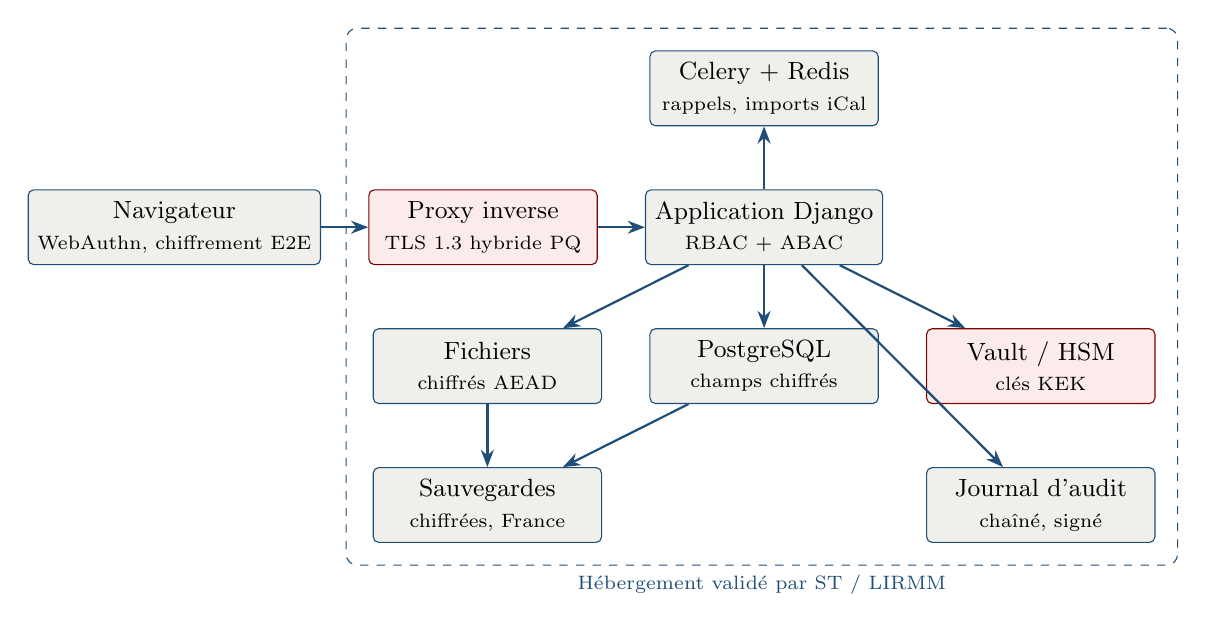
\begin{tikzpicture}[
  node distance=0.8cm and 0.6cm,
  box/.style={draw=bleu,rounded corners=2pt,fill=gris,align=center,
              minimum width=2.9cm,minimum height=0.95cm,font=\small},
  sec/.style={draw=red!50!black,rounded corners=2pt,fill=alerte,align=center,
              minimum width=2.9cm,minimum height=0.95cm,font=\small},
  arr/.style={-{Stealth[length=2.2mm]},thick,draw=bleu}]
  \node[box] (nav) {Navigateur\\\scriptsize WebAuthn, chiffrement E2E};
  \node[sec, right=of nav] (proxy) {Proxy inverse\\\scriptsize TLS 1.3 hybride PQ};
  \node[box, right=of proxy] (app) {Application Django\\\scriptsize RBAC + ABAC};
  \node[box, below=of app] (db) {PostgreSQL\\\scriptsize champs chiffrés};
  \node[box, left=of db] (files) {Fichiers\\\scriptsize chiffrés AEAD};
  \node[sec, right=of db] (kms) {Vault / HSM\\\scriptsize clés KEK};
  \node[box, above=of app] (worker) {Celery + Redis\\\scriptsize rappels, imports iCal};
  \node[box, below=of files] (bak) {Sauvegardes\\\scriptsize chiffrées, France};
  \node[box, below=of kms] (log) {Journal d'audit\\\scriptsize chaîné, signé};
  \draw[arr] (nav) -- (proxy);
  \draw[arr] (proxy) -- (app);
  \draw[arr] (app) -- (db);
  \draw[arr] (app) -- (files);
  \draw[arr] (app) -- (kms);
  \draw[arr] (app) -- (worker);
  \draw[arr] (db) -- (bak);
  \draw[arr] (files) -- (bak);
  \draw[arr] (app) -- (log);
  \begin{scope}[on background layer]
    \node[draw=bleu,dashed,rounded corners,inner sep=8pt,
          fit=(proxy)(app)(db)(files)(kms)(worker)(bak)(log),
          label={[font=\scriptsize,text=bleu]below:Hébergement validé par ST / LIRMM}] {};
  \end{scope}
\end{tikzpicture}
\end{center}

\noindent Déploiement : Docker Compose sur un serveur interne, Caddy ou Nginx en
façade, intégration continue avec tests de sécurité, mises à jour automatiques des
dépendances.

\subsection{Feuille de route}
\begin{enumerate}
  \item \textbf{Nov.--déc.\ 2026 : cadrage.} Présenter ce document au directeur et au
  tuteur ST ; obtenir leur avis sur l'hébergement et la confidentialité.
  \item \textbf{Janv.--févr.\ 2027 : MVP.} Modules 1, 3, 4 et 5 ; authentification
  WebAuthn ; TLS hybride ; chiffrement par enveloppe.
  \item \textbf{Mars 2027 : mise en service.} Comptes des encadrants, objectifs de
  l'année 1 saisis à la première réunion.
  \item \textbf{Printemps--été 2027.} Module 6, journal de bord, registre des décisions,
  signatures des validations.
  \item \textbf{Avant mars 2028.} Génération du premier rapport ANRT et du dossier CSI ;
  chiffrement de bout en bout du niveau confidentiel.
  \item \textbf{Années 2 et 3.} Ajustements selon l'usage réel ; passage aux signatures
  hybrides ML-DSA ; export du dossier de soutenance.
\end{enumerate}

\begin{question}[Questions à poser aux encadrants]
\begin{itemize}[leftmargin=*]
  \item[$\square$] ST autorise-t-elle un outil hébergé hors de son réseau, même pour les
  seules données non techniques ?
  \item[$\square$] Qui, au LIRMM, valide l'hébergement d'un outil manipulant des
  informations de la ZRR ?
  \item[$\square$] Quel est le délai de relecture interne d'une publication chez ST ?
  \item[$\square$] Quelle répartition de temps figure dans le contrat de collaboration ?
  \item[$\square$] L'ED I2S exige-t-elle un CSI dès la réinscription de septembre 2027 ?
\end{itemize}
\end{question}

% =====================================================================
\section*{Sources}
\addcontentsline{toc}{section}{Sources}
% =====================================================================
\small
\paragraph{Réglementation doctorale.}
\href{https://www.legifrance.gouv.fr/loda/id/JORFTEXT000032587086}{Arrêté du 25 mai 2016} ;
\href{https://www.legifrance.gouv.fr/jorf/id/JORFTEXT000046228965}{arrêté du 26 août 2022} ;
\href{https://edshal-docs.univ-cotedazur.fr/files/guide_CSI.pdf}{guide du CSI (RNCD)} ;
\href{https://direction-recherche.parisnanterre.fr/medias/fichier/guide-adum-csi_1696864722733-pdf}{guide ADUM du CSI (Paris Nanterre)} ;
\href{https://www.universite-paris-saclay.fr/convention-de-formation-doctorale}{convention de formation (Paris-Saclay)} ;
\href{https://www.imt-mines-ales.fr/sites/default/files/media/2020-09/charte_du_doctorat_i2s.pdf}{charte du doctorat I2S} ;
\href{https://www.umontpellier.fr/wp-content/uploads/2023/06/IDD_guide-inscription_V7.pdf}{guide d'inscription (Univ.\ de Montpellier)} ;
\href{https://www.cnam.fr/recherche-innovation/etudes-doctorales-hdr/soutenances}{soutenance et serment (Cnam)} ;
\href{https://u-paris.fr/doctorat/soutenir-sa-these/}{soutenance (Univ.\ Paris Cité)}.

\paragraph{CIFRE.}
\href{https://static.psl.eu/sites/default/files/2026-07/Webinaire\%20CIFRE\%20COFRA\%2007.04.26.pdf}{Webinaire PSL (2026)} ;
\href{https://ed-lls.parisnanterre.fr/medias/fichier/presentation-cifre-cofra_1776946105660-pdf}{présentation Paris Nanterre (2026)} ;
\href{https://www.universita.corsica/actus/userfiles/file/RECHERCHE/Ecole\%20Doctorale/CIFRE_conditions_octroi_02_2009.pdf}{conditions générales d'octroi}.

\paragraph{LIRMM et ZRR.}
\href{https://www.lirmm.fr/?p=3918}{Doctorat au LIRMM} ;
\href{https://www.lirmm.fr/?p=1097}{HAL-LIRMM} ;
\href{https://armement.defense.gouv.fr/sites/default/files/2025-05/Instruction\%20interminist\%C3\%A9rielle_20250428_PPST.pdf}{instruction PPST (2025)} ;
\href{https://www.snesup.fr/sites/default/files/2025-11/recherche_snesup-ndeg-738pp22-23.pdf}{SNESUP n\textsuperscript{o}~738} ;
\href{https://armement.defense.gouv.fr/sites/default/files/2022-02/guide_ANSSI_protection_numerique_PSTN_juin_2018.pdf}{guide ANSSI ZRR}.

\paragraph{Plateformes et recherche.}
\href{https://studies.helsinki.fi/instructions/article/thessa}{Thessa} ;
\href{https://skillsforge.net}{SkillsForge} ;
\href{https://www.haplo.com/phd-manager}{Haplo} ;
\href{https://www.utwente.nl/en/service-portal/research-support/phd-engd-programmes-tgs/doctorate-phdengd-monitoring-system}{Doctorate (Twente)} ;
\href{https://hsd.ardascience.com/index.php/journal/article/download/1623/264/5253}{ProGRess} ;
\href{https://ajet.org.au/index.php/AJET/article/download/8615/2025/30010}{Fanshawe et Barton (2023)}.

\paragraph{Conférences.}
\href{https://easychair.org/cfp/pqcrypto2027}{PQCrypto 2027} ;
\href{https://tches.iacr.org/index.php/TCHES/submission}{TCHES} ;
\href{https://gdr-securite.irisa.fr/evenement/cascade-2025}{CASCADE} ;
\href{https://www.iacr.org/events/eventsbysubmission.php4}{calendrier IACR} ;
\href{https://sec-deadlines.github.io}{sec-deadlines}.

\paragraph{Cryptographie.}
\href{https://csrc.nist.gov/pubs/fips/203/final}{FIPS 203 (ML-KEM)} ;
\href{https://csrc.nist.gov/pubs/fips/204/final}{FIPS 204 (ML-DSA)} ;
\href{https://owasp.org/www-project-application-security-verification-standard/}{OWASP ASVS}.

\end{document}
